\chapter{IMPLEMENTASI}
Pada bab ini akan dipaparkan implementasi dari sistem yang dibangun. Bahasa pemrograman yang digunakan adalah HTML, CSS, Javascript, dan PHP yang dikemas dalam framework Laravel.

\section{Lingkungan Implementasi}
\tab Lingkungan implementasi dalam pembuatan sistem pada Kerja Praktik kali ini meliputi perangkat keras dan perangkat lunak yang digunakan untuk mengimplementasikan sistem yang telah dirancang adalah sebagai berikut:
\begin{enumerate}
	\item Perangkat Keras
	\begin{itemize}
	\item \textit{Processor} Intel(R) Core(IM i3-330M @ 2.13GHz
	\item Memori 4 GB
	\end{itemize}
	\item Perangkat Lunak
	\begin{itemize}
	\item Sistem Operasi Windows 10 64 bit.
	\item \textit{Text editor} Jetbrains PHPstorm.
	\item Bahasa pemrograman PHP.
	\end{itemize}
\end{enumerate}

\section{Tampilan Fitur Aplikasi Monitoring SIK}
Berikut adalaha tampilan aplikasi \textit{monitoring} SIK.
\subsection{Halaman \textit{Dashboard} \textit{Monitoring} SIK}
Pada halaman tampilan \textit{dashboard Monitoring} SIK ini menggunakan HTML, CSS dan PHP untuk tampilan sistem. Penampilan data pada halaman ini bersifat dinamis. Semua fitur pada aplikasi \textit{Monitoring} SIK didaftar secara rinci dan dikemas dalam tampilan \textit{grid}. Kemudian ketika salah satu fitur dipilih oleh user, maka akan diarahkan pada halaman sesuai fitur yang dipilih. Gambar \ref{lst:dashboard} adalah potongan kode dari halaman \textit{dashboard Monitoring} SIK.

\lstinputlisting[language=PHP, firstline=19, lastline=38, firstnumber=1, caption=Potongan Kode Tampilan \textit{Dashboard Monitoring} SIK, label={lst:dashboard}]{bab5/src/MainController.php}

\subsection{Tampilan Halaman Menambahkan \textit{Request} Relokasi}
Pada halaman menambahkan \textit{request} relokasi menggunakan HTML, CSS, PHP dan Javascript. Sebuah \textit{form} ditampilkan kemudian user mengisikan data-data yang diperlukan. \textit{Form} tersebut akan menampung data-data yang diperlukan, kemudian akan disimpan ke dalam basis data sistem. Gambar \ref{figure:tambahReqRelokasi} adalah tampilan dan gambar \ref{lst:addrelokasi1}, \ref{lst:addrelokasi2} dan \ref{lst:addrelokasi3} adalah potongan kode halaman menambahkan \textit{request} relokasi.
\begin{figure}[h!]
\centerline
{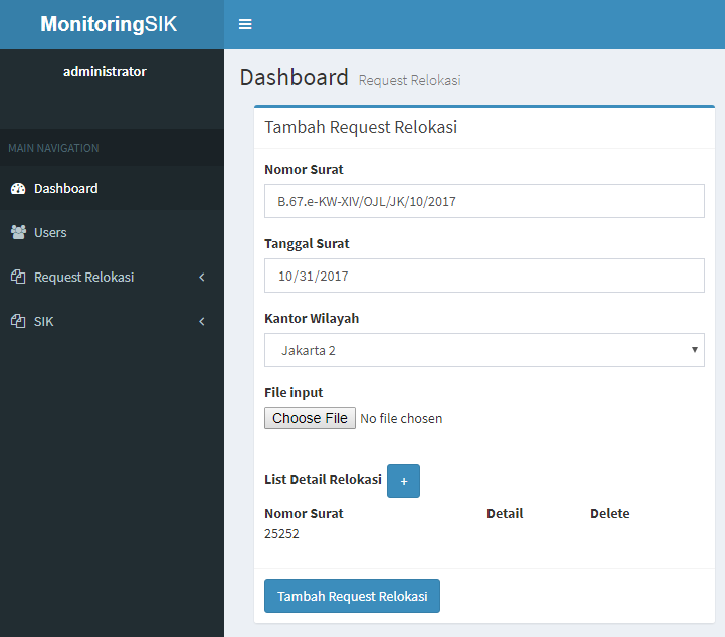
\includegraphics[width=10cm,height=7.5cm]{bab5/addReqRelokasi.png}}
\caption{Potongan Halaman Menambahkan \textit{Request} Relokasi}
\label{figure:tambahReqRelokasi}
\end{figure}

\lstinputlisting[language=PHP, firstline=34, lastline=45, firstnumber=1, caption=Potongan Kode Tampilan Menambahkan \textit{Request} Relokasi (1), label={lst:addrelokasi1}]{bab5/src/RelocationRequestController.php}
\lstinputlisting[language=PHP, firstline=46, lastline=82, firstnumber=14, caption=Potongan Kode Tampilan Menambahkan \textit{Request} Relokasi (2), label={lst:addrelokasi2}]{bab5/src/RelocationRequestController.php}
\lstinputlisting[language=PHP, firstline=83, lastline=109, firstnumber=51, caption=Potongan Kode Tampilan Menambahkan \textit{Request} Relokasi (3), label={lst:addrelokasi3}]{bab5/src/RelocationRequestController.php}

\subsection{Tampilan Halaman Menambahkan SIK}
Pada halaman menambahkan SIK menggunakan HTML, CSS, PHP dan Javascript. Sebuah \textit{form} ditampilkan kemudian user mengisikan data-data yang diperlukan. \textit{Form} tersebut akan menampung data-data yang diperlukan, kemudian akan disimpan ke dalam basis data sistem. Pada pengisian nomor \textit{request} relokasi, didapatkan dari \textit{record} pada basis data sistem. Gambar \ref*{figure:tambahSIK} adalah tampilan dan gambar \ref{lst:addSIK1} dan \ref{lst:addSIK2} adalah potongan kode dari halaman menambahkan SIK.
\begin{figure}[h!]
\centerline
{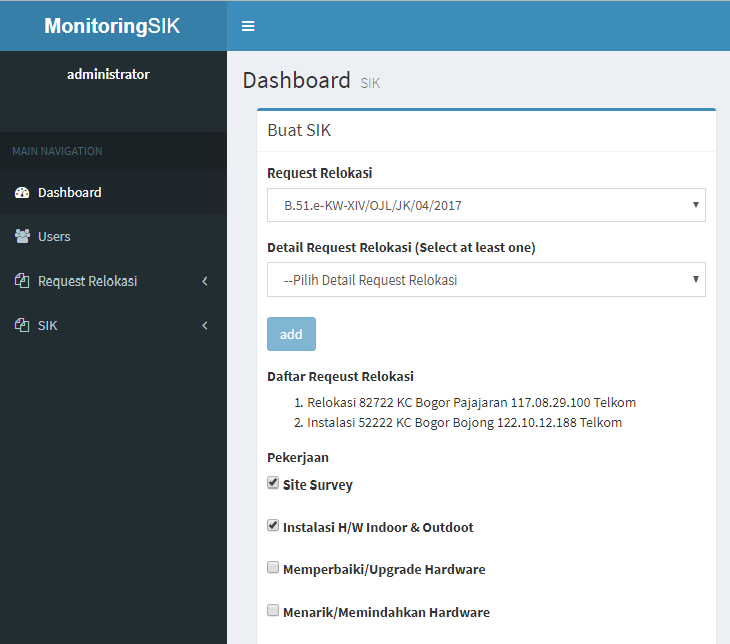
\includegraphics[width=10cm,height=6cm]{bab5/addSIK.png}}
\caption{Potongan Halaman Menambahkan SIK}
\label{figure:tambahSIK}
\end{figure}

\lstinputlisting[language=PHP, firstline=72, lastline=86, firstnumber=1, caption=Potongan Kode Tampilan Menambahkan SIK(1), label={lst:addSIK1}]{bab5/src/WorkPermitController.php}
\lstinputlisting[language=PHP, firstline=87, lastline=110, firstnumber=18, caption=Potongan Kode Tampilan Menambahkan SIK(2), label={lst:addSIK2}]{bab5/src/WorkPermitController.php}

\subsection{Halaman Detail SIK}
Pada halaman detail SIK menggunakan HTML, CSS dan PHP. Pada halaman ini, user dapat melihat rincian pekerjaan yang akan dilakukan pada permintaan relokasi yang telah dibuat, dan keterangan-keterangan lain seperti PIC pengerjaan, Nomor Surat Perintah Kerja, dan informasi-infromasi lain. Halaman detail SIK ini juga memungkinkan admin menambahkan eksekusi, dengan cara mengubah status pengerjaan proyek. Tombol \textit{accept} hanya dapat digunakan apabila user telah meng\textit{upload} surat SIK yang telah disetujui oleh Kepala Divisi. Gambar \ref{lst:detailSIK} adalah potongan kode dari halaman detail SIK.

\lstinputlisting[language=PHP, firstline=66, lastline=74, firstnumber=1, caption=Potongan Kode Tampilan Detail SIK, label={lst:detailSIK}]{bab5/src/WorkPermitController.php}

\subsection{Halaman Detail Eksekusi}
Pada halaman detail Eksekusi menggunakan HTML, CSS dan PHP. Pada halaman ini, user dapat melihat rincian pekerjaan yang akan dilakukan pada permintaan relokasi. Halaman detail eksekusi ini juga memungkinkan admin menambahkan penagihan, dengan cara mengubah status pengerjaan proyek. Tombol selesai hanya dapat digunakan apabila user telah meng\textit{upload} berita acara dan tagihan yang diberikan oleh pihak provider. Gambar \ref{lst:detailEksekusi} adalah potongan kode dari halaman detail eksekusi.

\lstinputlisting[language=PHP, firstline=70, lastline=78, firstnumber=1, caption=Potongan Kode Tampilan Detail Eksekusi, label={lst:detailEksekusi}]{bab5/src/ExecutionController.php}

\subsection{Halaman Detail Penagihan}
Pada halaman detail Penagihan menggunakan HTML, CSS dan PHP. Pada halaman ini, user dapat melihat proses penagihan dan pembayaran. Halaman detail SIK ini juga memungkinkan admin menambahkan proses finish, dengan cara mengubah status pembayaran proyek. Tombol selesai hanya dapat digunakan apabila user telah meng\textit{upload} surat pengantar pembayaran kepada pihak provider. Gambar \ref{lst:detailPenagihan} adalah potongan kode dari halaman detail penagihan.

\lstinputlisting[language=PHP, firstline=50, lastline=58, firstnumber=1, caption=Potongan Kode Tampilan Detail Penagihan, label={lst:detailPenagihan}]{bab5/src/BillingController.php}

\subsection{Halaman Detail \textit{Finish}}
Pada halaman detail Finish menggunakan HTML, CSS dan PHP. Pada halaman ini, user dapat melihat semua informasi yang berhubungan dengan pengerjaan proyek relokasi. Gambar \ref{lst:detailFinish1} dan \ref{lst:detailFinish2} adalah potongan kode dari halaman detail \textit{finish}.

\lstinputlisting[language=PHP, firstline=40, lastline=45, firstnumber=1, caption=Potongan Kode Tampilan Detail Finish(1), label={lst:detailFinish1}]{bab5/src/MainController.php}
\lstinputlisting[language=PHP, firstline=45, lastline=63, firstnumber=7, caption=Potongan Kode Tampilan Detail Finish(2), label={lst:detailFinish2}]{bab5/src/MainController.php} 